\subsection{Limitaciones de las Herramientas de Detección Actuales}

A pesar de los avances significativos en la detección de \glspl{url} maliciosas, las herramientas actuales aún enfrentan desafíos importantes. Los ciberdelincuentes continúan desarrollando técnicas más sofisticadas para crear clones de sitios web legítimos, lo que dificulta su detección incluso para las soluciones más avanzadas disponibles en el mercado.

\subsubsection{Problemas de Detección de Clones de Páginas Web}

Los clones de páginas web son versiones fraudulentas de sitios web legítimos, diseñadas para engañar a los usuarios y robar información confidencial. A continuación, se presentan ejemplos que ilustran este problema:





\begin{figure}[H]
    \centering
    
\includegraphics[width=0.8\textwidth]{discordReal.png}
    \caption{Página Original de Discord}
    \label{fig:original-discord}
\end{figure}

\begin{figure}[H]
    \centering
    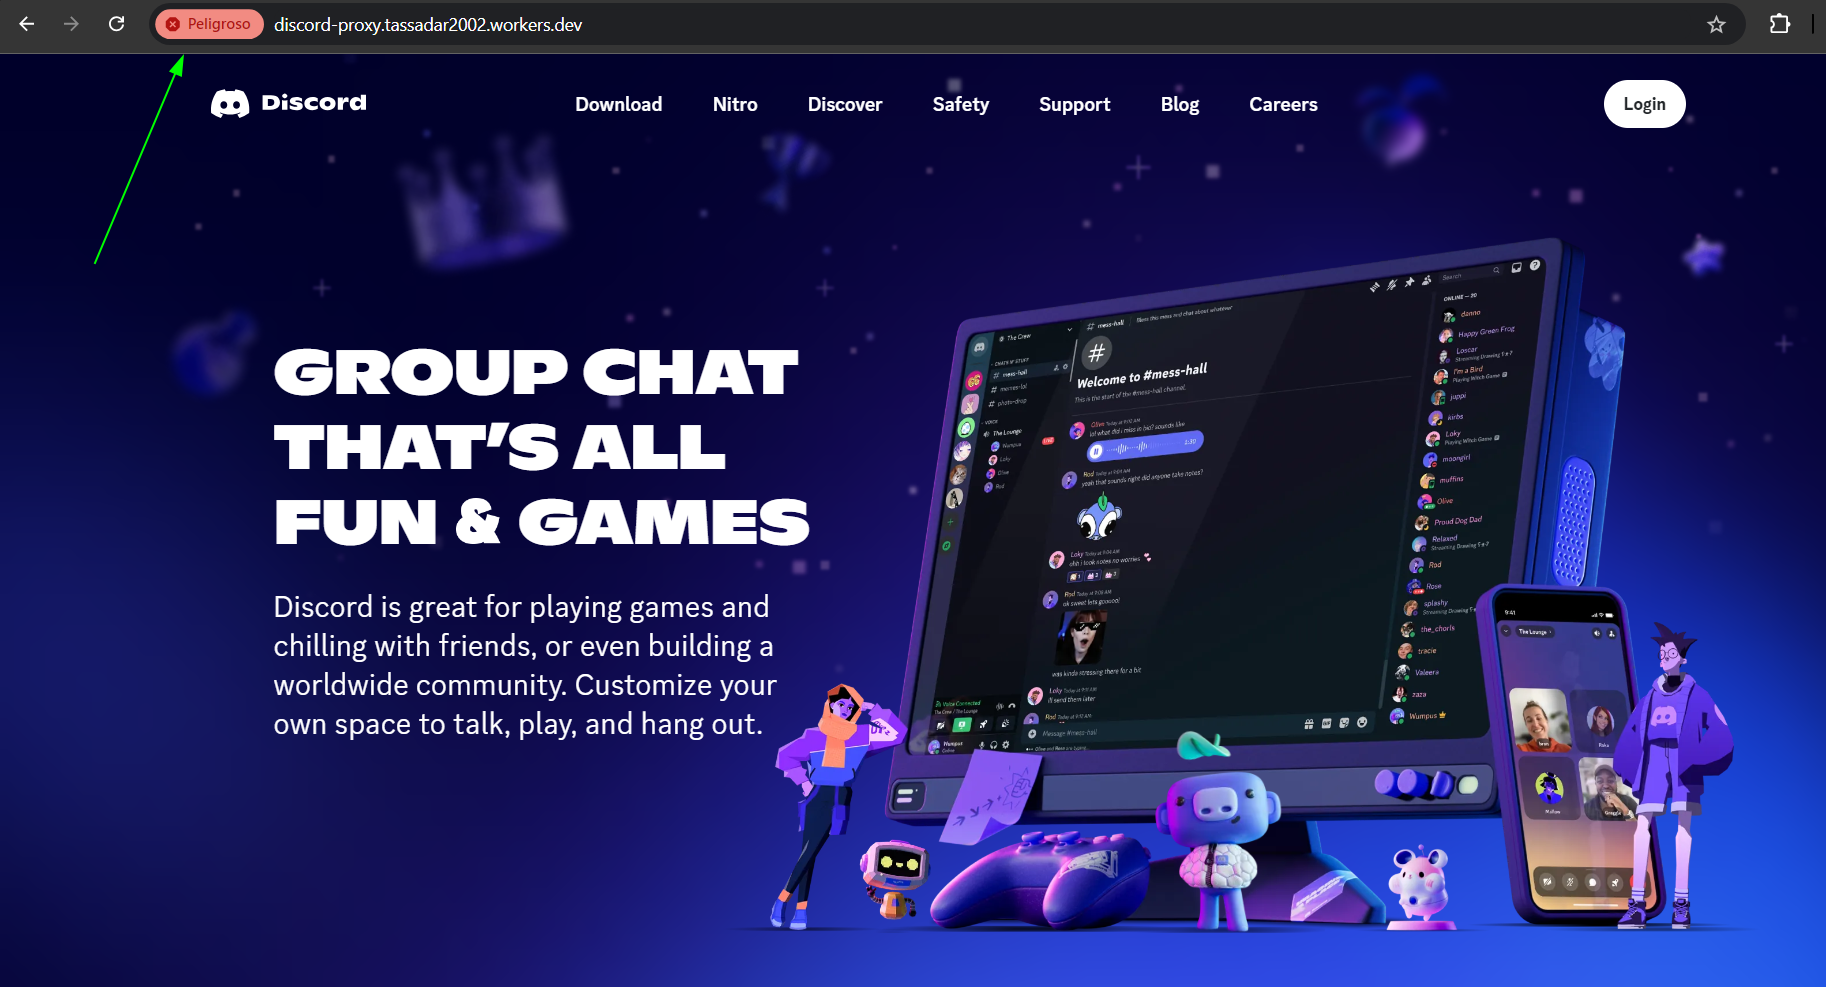
\includegraphics[width=0.8\textwidth]{discordFalso1.png}
    \caption{Clon de Discord Detectado por Google}
    \label{fig:google-detect-clone}
\end{figure}

\begin{figure}[H]
    \centering
    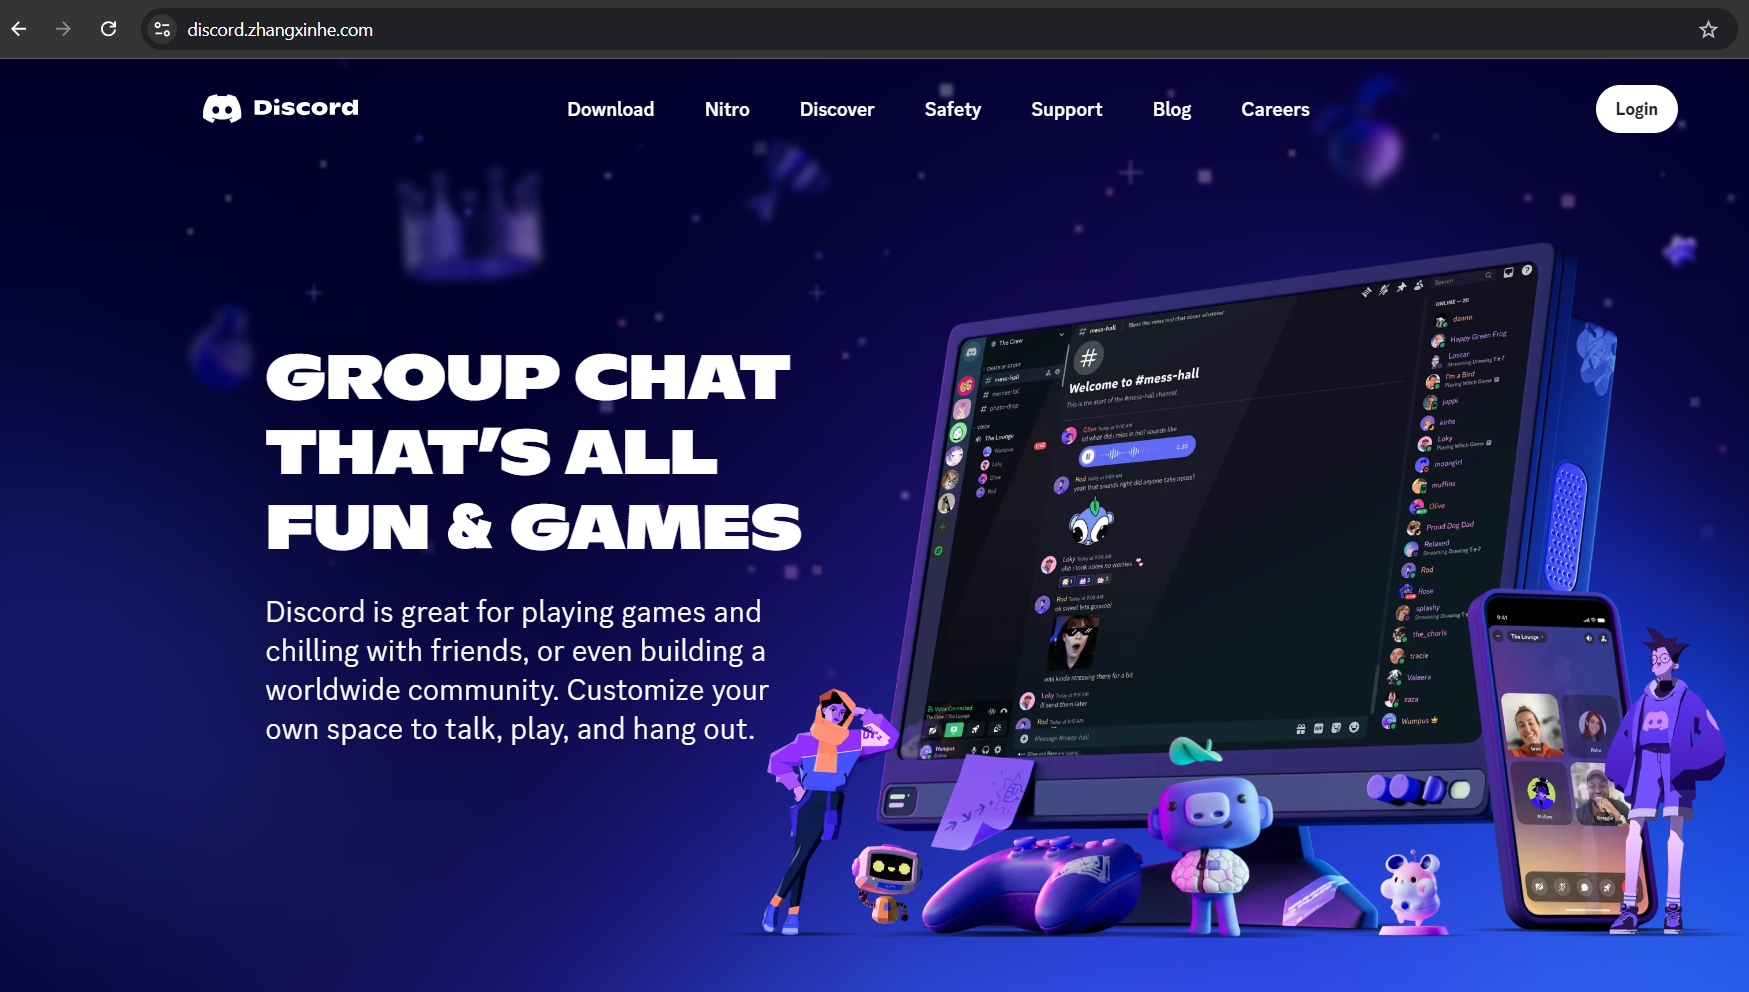
\includegraphics[width=0.8\textwidth]{discordFalso2.png}
    \caption{Clon de Discord No Detectado por Google}
    \label{fig:no-google-detect-clone}
\end{figure}

Estos ejemplos muestran que:

\begin{itemize}
    \item \textbf{Calidad del Clonado}: Los clones pueden ser extremadamente similares a las páginas legítimas, lo que los hace difíciles de detectar tanto para los usuarios como para los sistemas automatizados.
    \item \textbf{Eficacia de los Motores de Búsqueda}: Google puede detectar ciertos clones y advertir a los usuarios sobre su peligrosidad, pero no todos los clones son identificados, dejando una brecha de seguridad explotable.
    \item \textbf{Limitaciones de las Herramientas Actuales}: Herramientas de detección de phishing y malware pueden no ser infalibles. Los clones bien diseñados pueden evadir la detección, lo que pone en riesgo la seguridad del usuario.
\end{itemize}